% Created 2024-10-16 śro 21:35
% Intended LaTeX compiler: pdflatex
\documentclass[../main.tex]{subfiles}

% \usepackage[a4paper, margin=3cm]{geometry}
% \usepackage{amssymb} // not working

\usepackage[T1]{fontenc}
\usepackage[utf8]{inputenc}
\usepackage{graphicx}
\usepackage{longtable}
\usepackage{wrapfig}
\usepackage{rotating}
\usepackage[normalem]{ulem}
\usepackage{amsmath}
\usepackage{capt-of}
\usepackage{hyperref}
\usepackage{siunitx}
\usepackage{float}
\usepackage[polish]{babel}

\graphicspath{{../}}
\author{Wojciech Paderewski}
\date{\today}
\title{Dobór i test lamp nixie}
\hypersetup{
 pdfauthor={Wojciech Paderewski},
 pdftitle={Dobór i test lamp nixie},
 pdfkeywords={},
 pdfsubject={},
 pdflang={Polish}}

\begin{document}

Pierwszą rzeczą, która została wykonana to zakup lamp Nixie, które będą wykorzystane w projekcie. 
Przez coraz mniejszą dostępność lamp Nixie,
zdecydowano się na zakup małych lamp Z570M, które zostały zakupione w ilości 6 sztuk. Lampy te mają 10 cyfr oraz kropkę dziesiętną.
Lampy są używane, ale wszystkie lampy zostały sprawdzone i działają poprawnie.
Kluczowe parametry zastosowanych lamp nixie odczytane z karty katalogowej \cite{st:Z5730M} to:
\begin{itemize}
    \item Napięcie zapłonu: \SI{170}{\volt}
    \item Napięcie wygaszania: \SI{120}{\volt}
    \item Napięcie pracy: \SI{150}{\volt}
    \item Prąd katodowy średni: \SI{2}{\milli\ampere}
\end{itemize}

W celu zweryfikowania działania lamp nixie i sprawdzenia parametrów zasilania, został wykonany prototyp układu z jedną lampą nixie,
wykorzystujący zasilacz impulsowy wysokiego napięcia z regulowanym napięciem wyjściowym zakupiony w sklepie internetowym.

Zakupiona przetwornica wysokiego napięcia ma następujące parametry:
\begin{itemize}
    \item Napięcie wejściowe: \SI{5}-\SI{12}{\volt}
    \item Napięcie wyjściowe: \SI{150}-\SI{220}{\volt}
    \item Prąd wyjściowy: \SI{20}{\milli\ampere}
\end{itemize}

W celu sprawdzenia działania lampy należy najpierw dobrać rezystor ograniczający prąd katodowy.
Zakładając, że napięcie zasilania wynosi maksymalnie $U_{\text{max}} = \SI{220}{\volt}$, a napięciu pracy lampy $U_{\text{pr}} = \SI{150}{\volt}$,
przy prądzie katodowym $I_{\text{kat}} = \SI{2}{\milli\ampere}$, rezystor ograniczający prąd katodowy można obliczyć ze wzoru:

\begin{equation}
    R = \frac{U_{\text{max}} - U_{\text{pr}}}{I_{\text{kat}}} = \frac{\SI{220}{\volt} - \SI{150}{\volt}}{\SI{2}{\milli\ampere}} = \SI{35}{\kilo\ohm}
\end{equation}

W nocie katalogowej lampy nixie Z570M producent podaje, że zalecany rezystor ograniczający prąd katodowy 
powinien mieć wartość \SI{33}{\kilo\ohm} dla napięcie zasilania \SI{200}{\volt}, więc wartość \SI{35}{\kilo\ohm} dla napięcia \SI{220}{\volt}
wydaje się obliczona prawidłowo, taki też rezystor ma zostać użyty w faktycznym układzie.


Do testu użyto rezystora o wartości \SI{22}{\kilo\ohm} oraz rezystora o wartości \SI{10}{\kilo\ohm}, połączonych
szeregowo, co daje wartość \SI{32}{\kilo\ohm}, co jest wartością zbliżoną do obliczonej.

Z testów wynika, że lampy Nixie działają poprawnie, a dobrany rezystor ograniczający prąd katodowy jest odpowiedni. 
Przy napięciu zasilania \SI{150}{\volt} lampa świeci słabiej, ale jest to zgodne z oczekiwaniami. Natomiast przy napięciu \SI{220}{\volt} lampa świeci jasno i pojawiają się lekko niebieskie refleksy wewnątrz lampy, co jest zgodne z oczekiwaniami.

\begin{figure}[H]
    \centering
    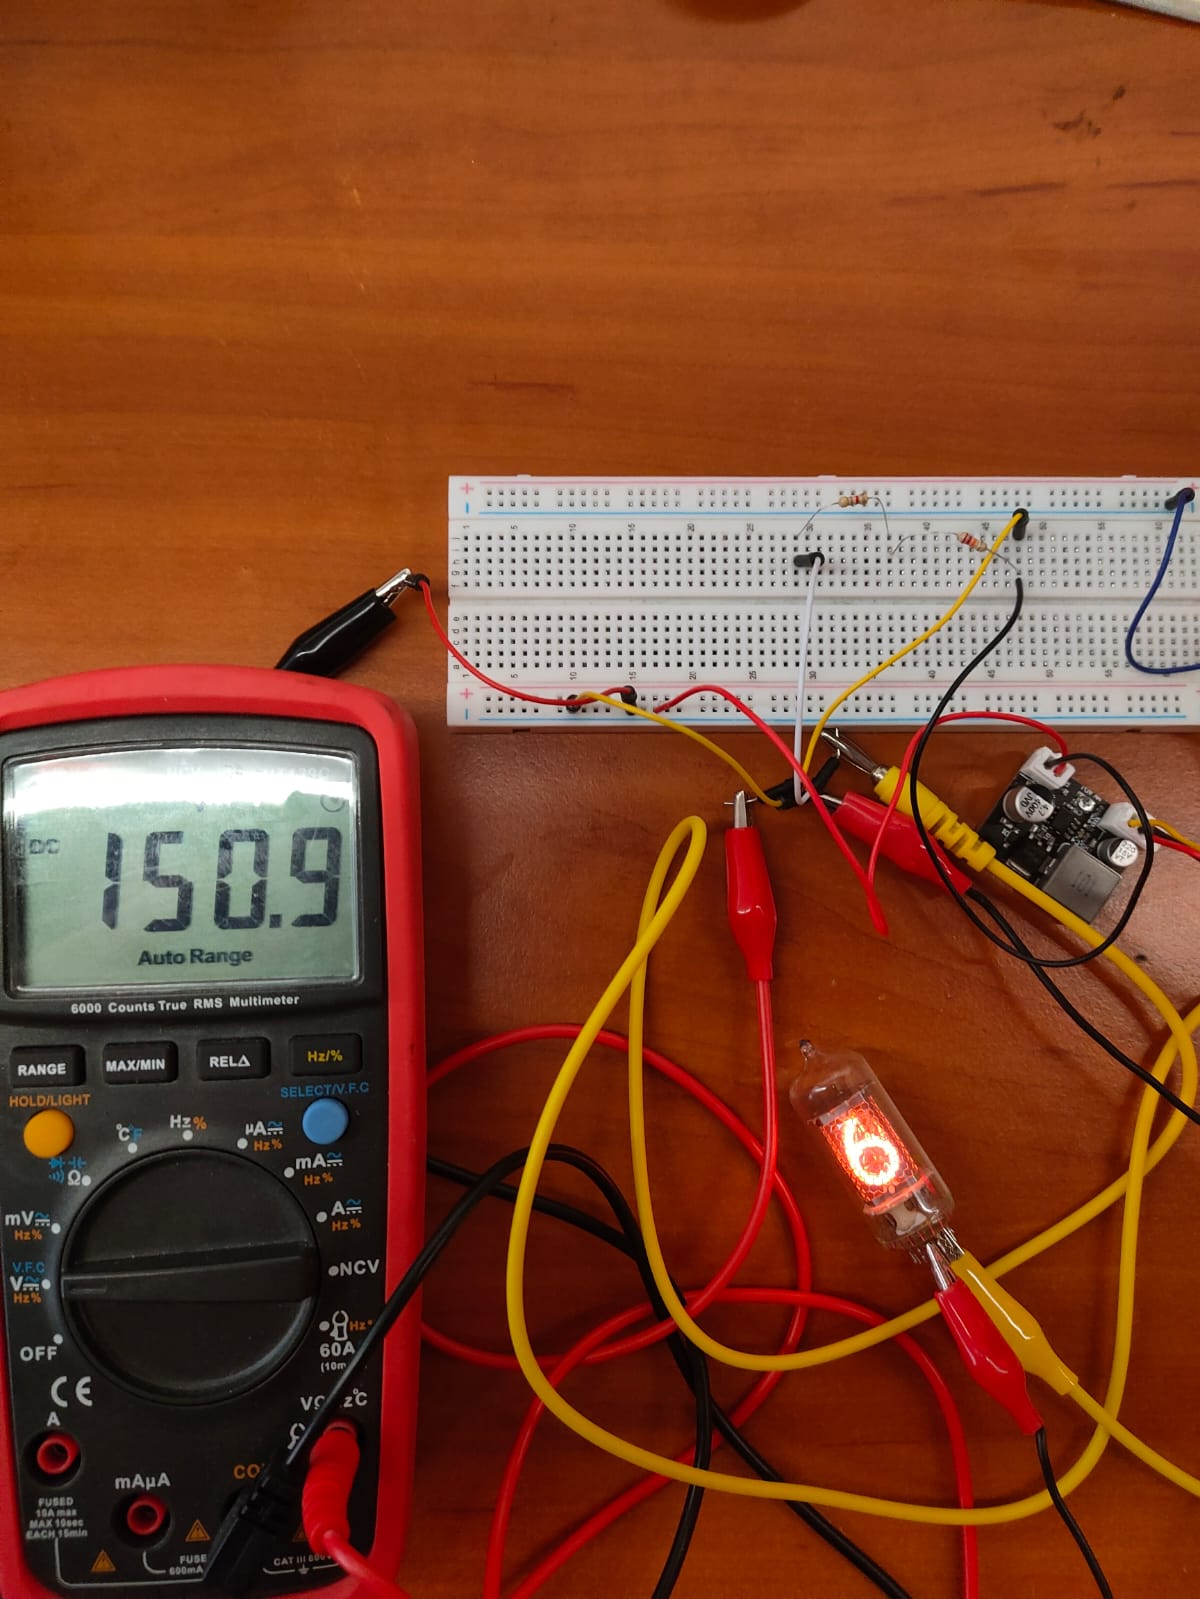
\includegraphics[width=0.4\textwidth]{nixie150V.jpeg}
    \caption{Prototyp układu z lampą Nixie przy napięciu zasilania \SI{150}{\volt}}
\end{figure}

\begin{figure}[H]
    \centering
    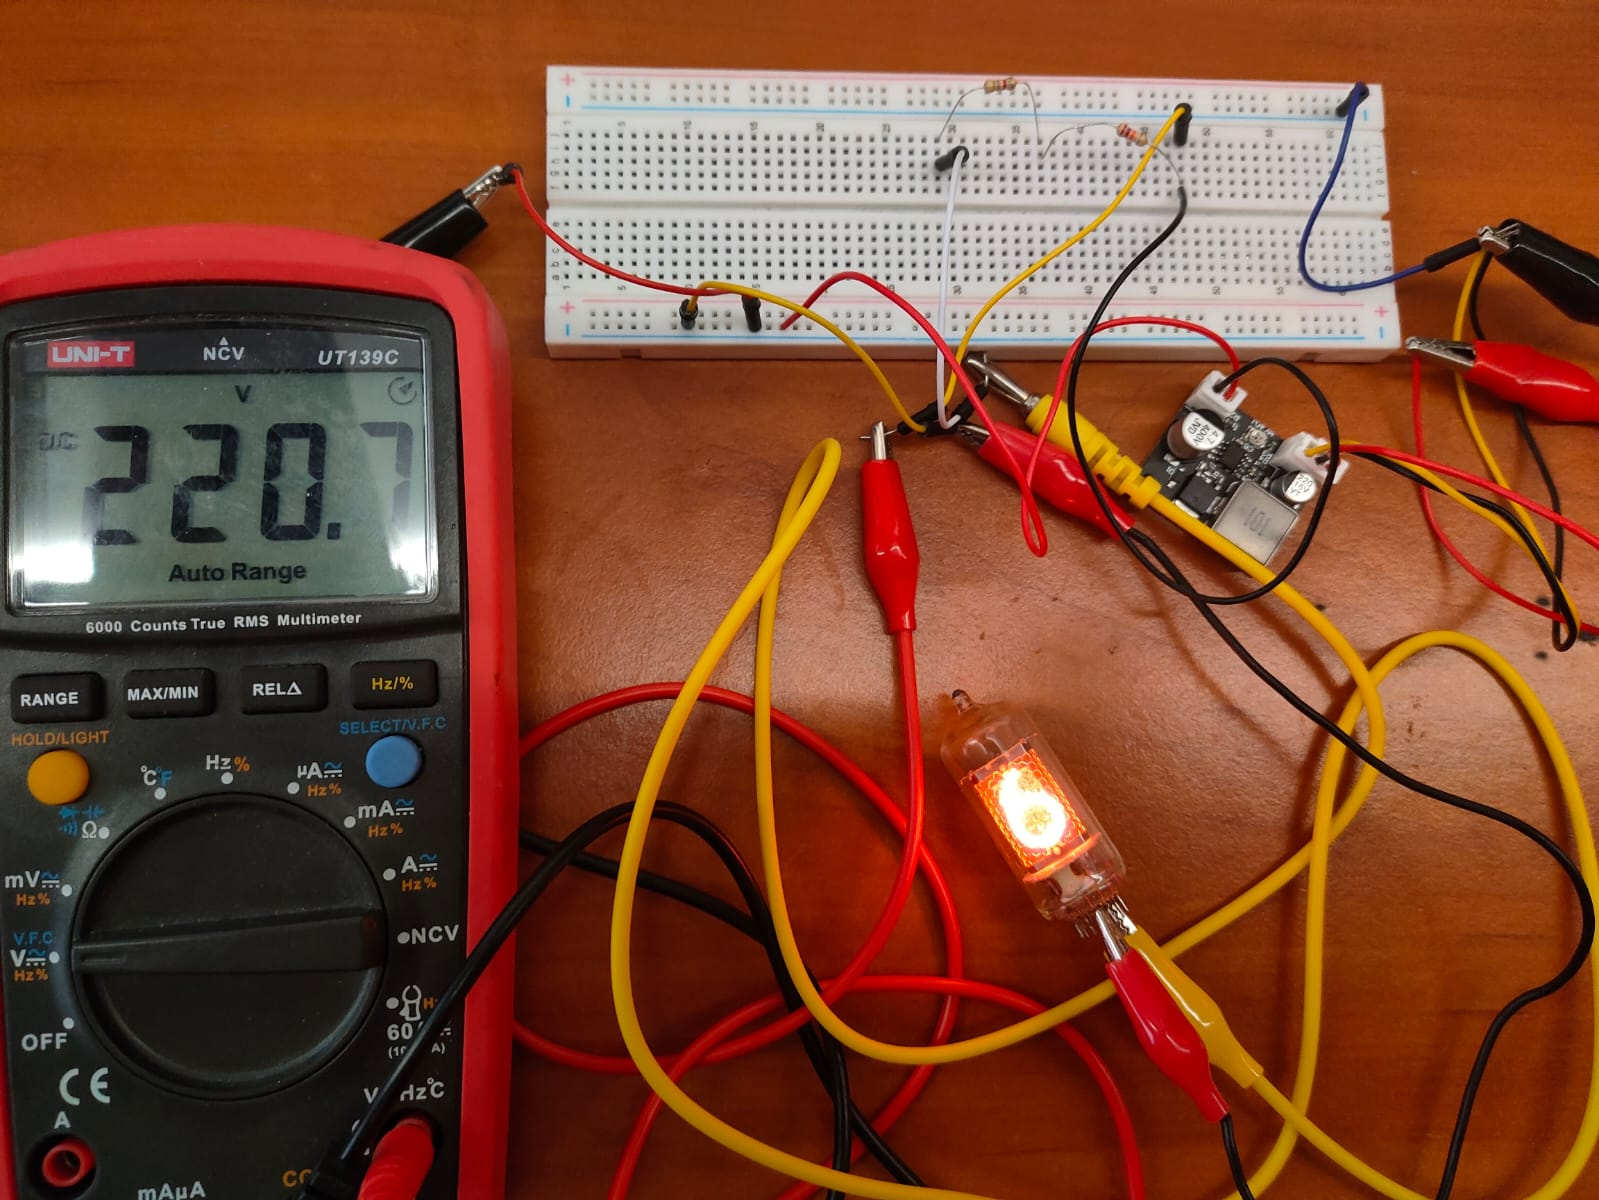
\includegraphics[width=0.5\textwidth]{nixie220V.jpeg}
    \caption{Prototyp układu z lampą Nixie przy napięciu zasilania \SI{220}{\volt}}
\end{figure}

Nie sprawdzono napięcia wygaszania, ponieważ zakres pracy zasilacza okazał się za mały. Ustalono jednak, że lampa nawet przy napięciu \SI{150}{\volt} była w stanie zapłonąć i świecić poprawnie.

Z testów można wyciągnąć następujące wnioski:

\begin{itemize}
    \item Lampy Nixie działają poprawnie przy napięciu zasilania \SI{150}{\volt} oraz \SI{220}{\volt}.
    \item Dobrany rezystor ograniczający prąd katodowy jest odpowiedni.
    \item Zakres regulacji napięcia powinien być większy, np. \SI{130}-\SI{220}{\volt}, by lampa mogła być jeszcze słabiej podświetlona. Może się to okazać przydatne w nocy.
\end{itemize}

\end{document}
